\makesectionpage[figures/ReinforcementLearning2.png]{Reinforcement Learning}

\begin{frame}{Reinforcement Learning: Grundidee}
\begin{columns}
\column{0.55\textwidth}
\begin{itemize}
  \item Neben überwachtem und unüberwachtem Lernen ist \textbf{Reinforcement
        Learning} das dritte große Lernparadigma.
  \item Ein \textbf{Agent} lernt durch \textbf{Interaktion} mit einer
        Umgebung.
  \item Er erhält für seine Handlungen eine \textbf{Belohnung} (Reward) als
        Rückmeldung.
  \item Ziel ist eine \textbf{Strategie}, die die Belohnung langfristig
        \textbf{maximiert}.
\end{itemize}

\column{0.40\textwidth}
\begin{blockC1}{Kernunterschied}
Es gibt keine gelabelten Beispiele. Der Agent lernt allein aus den
\textbf{Konsequenzen} seiner Handlungen.
\end{blockC1}


\begin{blockC2}{Voraussetzung}
Wir brauchen eine Umgebung, in der der Agent \textbf{gefahrlos trainieren} kann  (z.~B. ein Simulator).
\end{blockC2}



\end{columns}
\source{\cite{Frochte2020}}
\end{frame}

\begin{frame}{Reinforcement Learning: Agent und Umgebung}
\begin{columns}
\column{0.40\textwidth}
\begin{itemize}
  \item Der \textbf{Agent} wählt in jedem Schritt eine \textbf{Aktion}.
  \item Die \textbf{Umgebung} antwortet mit einem neuen \textbf{Zustand} und
        einer \textbf{Belohnung}.
  \item Aus dieser Schleife lernt der Agent seine \textbf{Strategie}.
\end{itemize}

\column{0.55\textwidth}
\centering
\resizebox{\linewidth}{!}{%
\begin{tikzpicture}[>=Stealth,
  box/.style={rectangle, rounded corners, draw=SecondaryTitle,
              fill=SecondaryColor, very thick, text=white,
              minimum width=2.4cm, minimum height=1.1cm,
              font=\bfseries, align=center}
]
% Boxen
\node[box] (agent) at (0,2) {Agent};
\node[box, fill=AccentColor, draw=AccentTitle] (env) at (0,-2) {Umgebung};
% Aktion (rechts herum)
\draw[->, very thick, SecondaryTitle]
  (agent.east) to[bend left=45]
  node[right, font=\footnotesize, text=black, align=left]
  {Aktion $a_t$} (env.east);
% Zustand + Reward (links herum)
\draw[->, very thick, AccentTitle]
  (env.west) to[bend left=45]
  node[left, font=\footnotesize, text=black, align=right]
  {Zustand $s_{t+1}$\\Belohnung $r_{t+1}$} (agent.west);
\end{tikzpicture}}
\end{columns}
\source{\cite{Frochte2020}}
\end{frame}

\begin{frame}{Reinforcement Learning: Grundbegriffe}
\begin{columns}
\column{0.55\textwidth}
\begin{itemize}
  \item \textbf{Zustand} $s_t$: die aktuelle Situation der Umgebung.
  \item \textbf{Aktion} $a_t$: die vom Agenten gewählte Handlung.
  \item \textbf{Belohnung} $r_{t+1}$: die Rückmeldung nach der Aktion.
  \item \textbf{Strategie} $\pi$: die Regel, die jedem Zustand eine Aktion
        zuordnet.
\end{itemize}

\column{0.40\textwidth}
\begin{block}{Ablauf pro Schritt}
Der Agent beobachtet $s_t$, wählt $a_t$ nach $\pi$, erhält $r_{t+1}$ und
landet in $s_{t+1}$.
\end{block}
\end{columns}
\source{\cite{Frochte2020}}
\end{frame}



\begin{frame}{Reinforcement Learning: Hundetraining als Beispiel}
\begin{columns}
\column{0.47\textwidth}
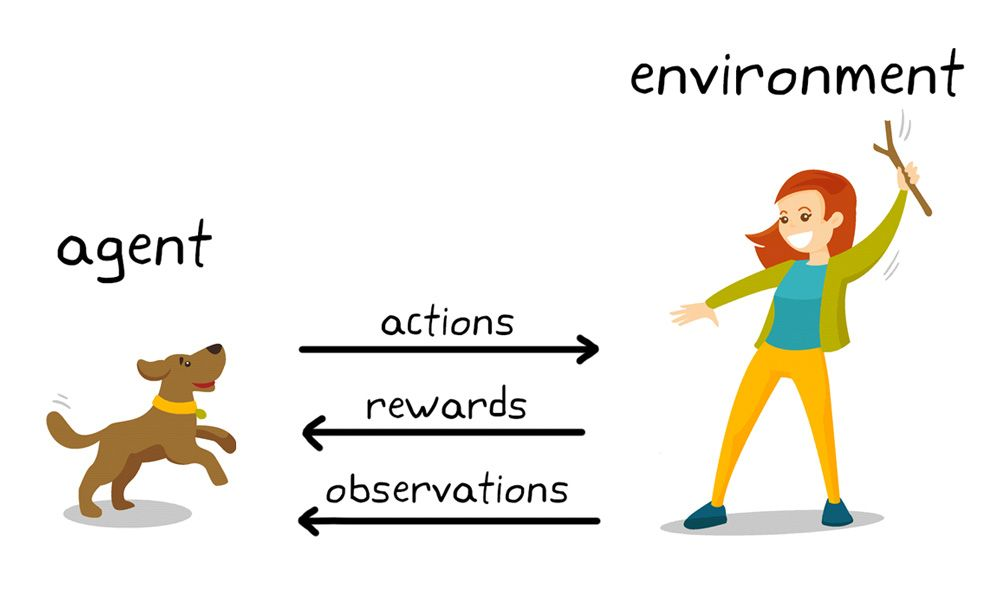
\includegraphics[width=\linewidth]{figures/reinforcement_hund.jpg}

\column{0.48\textwidth}
\begin{itemize}
\item \textbf{Agent:} Der Hund, der trainiert wird
\item \textbf{Environment:} Trainingsumgebung inkl. Trainerin und Stock
\item \textbf{Action:} Reaktion des Hundes (z.\,B. Stock apportieren)
\item \textbf{State:} Aktueller Lernzustand des Hundes
\begin{itemize}
\item kann Aufgabe bereits?
\item noch unsicher?
\end{itemize}
\item \textbf{Reward:}
\begin{itemize}
\item positiv: Leckerchen
\item neutral: keine Belohnung
\item negativ: Korrektur
\end{itemize}
\end{itemize}
\end{columns}
\source{\cite{Tzorakoleftherakis2020}, Bildquelle: \cite{Tzorakoleftherakis2020}}
\end{frame}


\begin{frame}{Anwendungsfälle von Reinforcement Learning}
\footnotesize



\begin{columns}[T]

    \column{0.5\textwidth}
\begin{itemize}
\item \textbf{Robotik:}
\begin{itemize}
\item Planung von Bewegungsabläufen
\item Lernen neuer Fähigkeiten
\item Interaktion mit realer Umgebung
\end{itemize}
\end{itemize}

\column{0.5\textwidth}
\begin{itemize}
\item \textbf{Spiele:}
\begin{itemize}
\item wenige Aktionen, klar definierte Zustände $\rightarrow$ \textbf{ideal} für RL
\item Agenten besser als Experten
\item Beispiele: Schach, Go, StarCraft~II
\end{itemize}
\end{itemize}


\end{columns}

\vspace{0.3cm}

\begin{columns}[T]
\column{0.5\textwidth}
\begin{center}
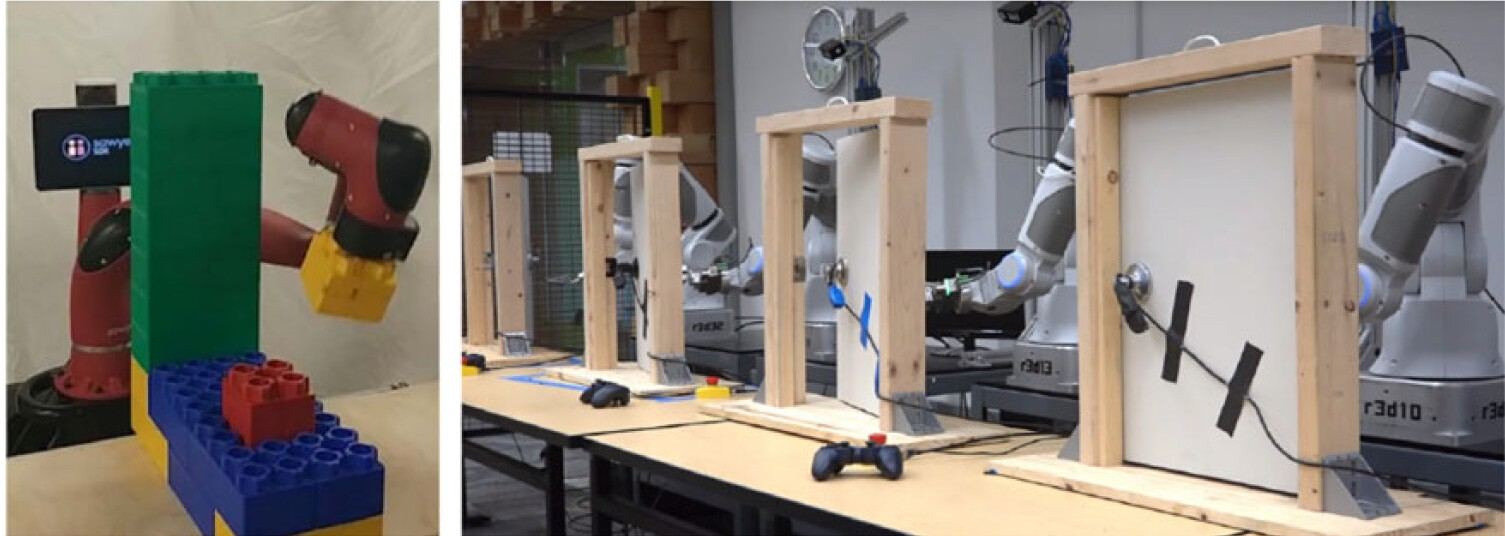
\includegraphics[width=1.0\linewidth]{figures/reinforce_robot.jpg}\\*[0.5ex]
\scriptsize Roboter spielen Lego und öffnen Türen \tiny (Bildquelle: \cite{Ibarz2021})
\end{center}

\column{0.4\textwidth}
\begin{center}
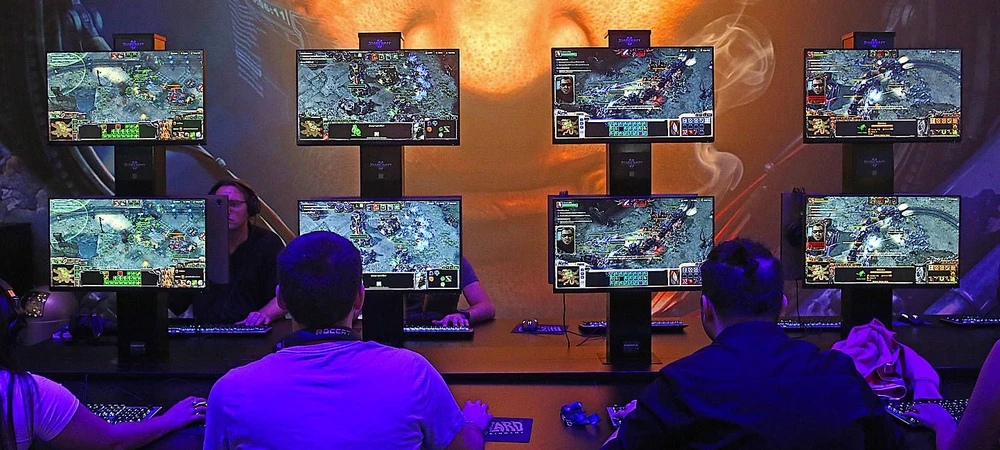
\includegraphics[width=1.0\linewidth]{figures/reinforce_star_craft.png}\\*[0.5ex]
\scriptsize AlphaStar besiegt besten StarCraft~II Spieler der Welt \tiny (Bildquelle: \cite{FAZ2019DeepMind})
\end{center}
\end{columns}

\source{\cite{Taulli2022,Datasolut2024,Ibarz2021}}
\end{frame}

\begin{frame}{Reinforcement Learning: Markov-Entscheidungsprozess}
\begin{columns}
\column{0.5\textwidth}
Das Zusammenspiel wird als \textbf{Markov-Entscheidungsprozess} (MDP)
modelliert, beschrieben durch:
\begin{itemize}
  \item eine Menge von \textbf{Zuständen} $S$,
  \item eine Menge von \textbf{Aktionen} $A$,
  \item eine \textbf{Übergangswahrscheinlichkeit}
        $P(s' \mid s, a)$,
  \item eine \textbf{Belohnungsfunktion} $R(s, a)$.
\end{itemize}

\column{0.40\textwidth}
\begin{blockC1}{Markov-Eigenschaft}
Der nächste Zustand hängt \textbf{nur} vom aktuellen Zustand und der Aktion
ab, nicht von der Vergangenheit.
\end{blockC1}
\end{columns}
\source{\cite{Frochte2020}}
\end{frame}

\begin{frame}{Umsetzung von Reinforcement Learning}
\begin{columns}
\begin{column}{0.4\textwidth}
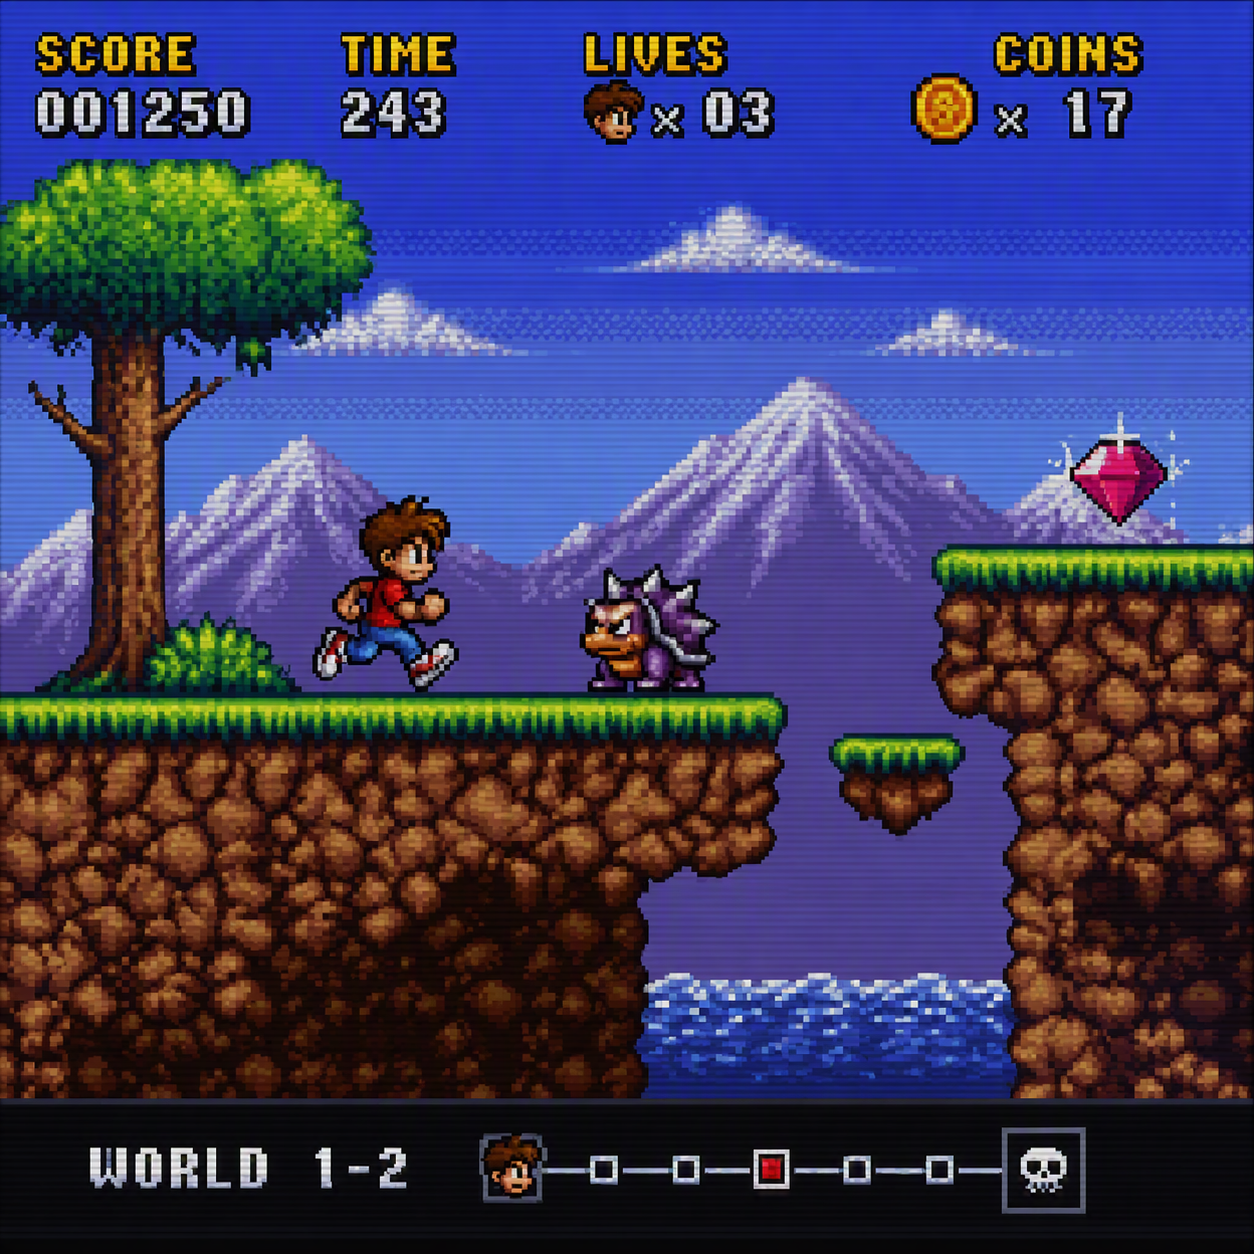
\includegraphics[width=\linewidth]{figures/jump_and_run.png}
\end{column}
\begin{column}{0.55\textwidth}
Wir betrachten ein \textbf{Jump-and-Run-Spiel}.
\begin{itemize}
\item Wie lässt sich der \textbf{State} beschreiben?
\item Welche \textbf{Actions} sind möglich?
\end{itemize}
\end{column}
\end{columns}
\source{\cite{seemann2024mlaz}}
\end{frame}

\begin{frame}{State und Actions im Jump-and-Run}
\begin{columns}
\begin{column}{0.4\textwidth}
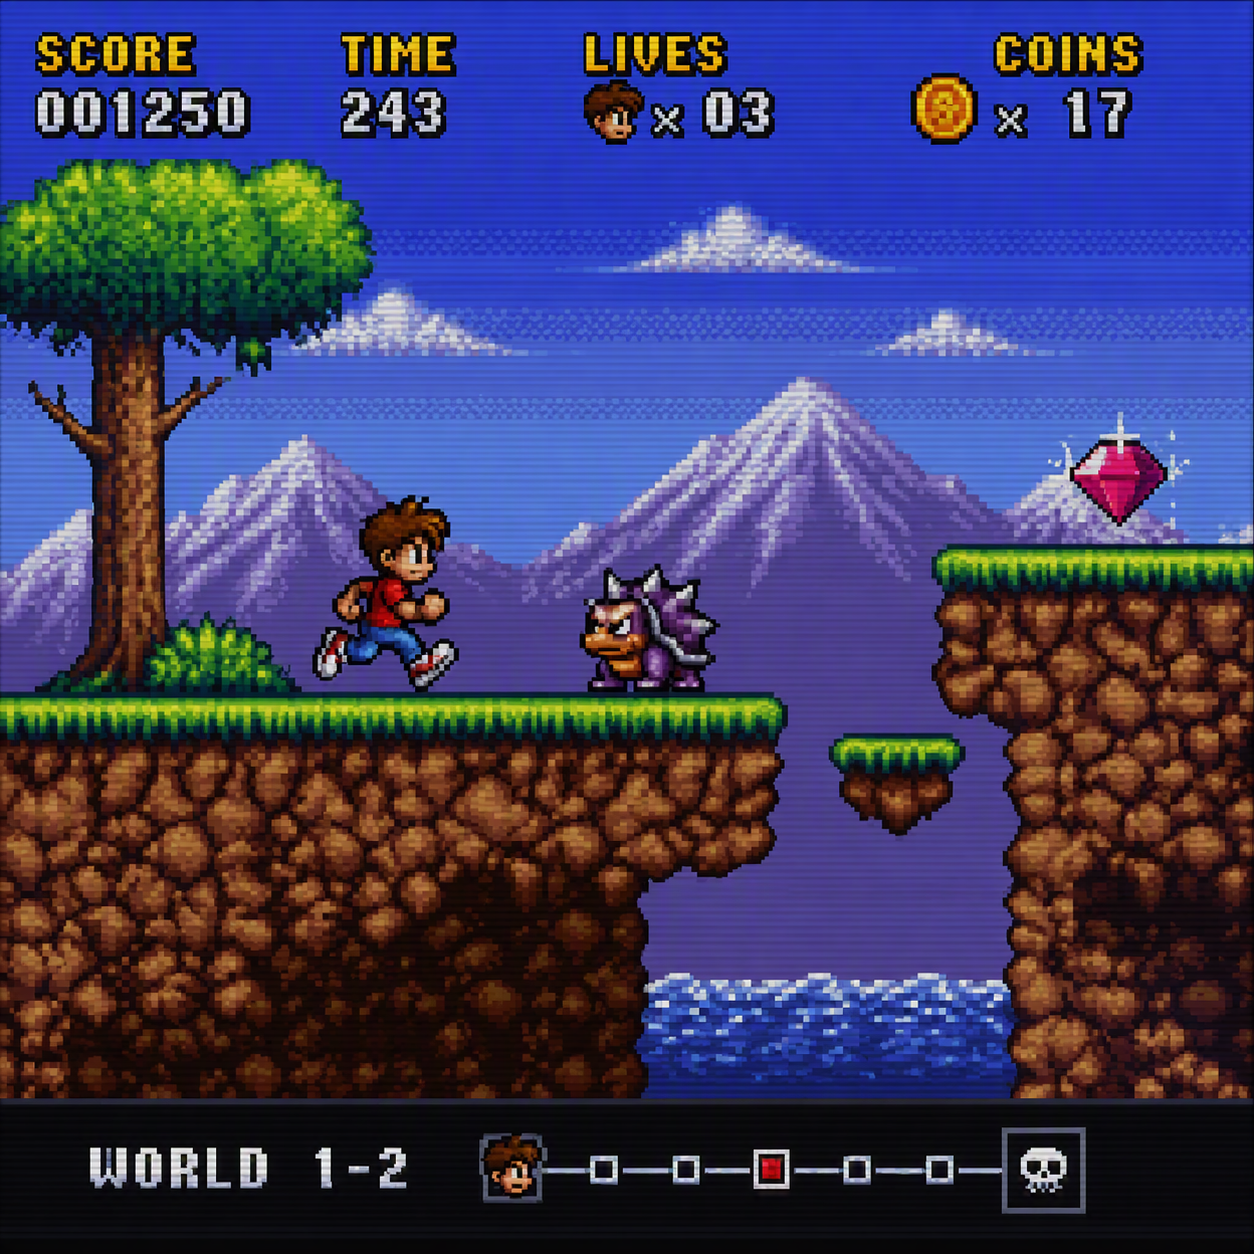
\includegraphics[width=\linewidth]{figures/jump_and_run.png}
\end{column}
\begin{column}{0.55\textwidth}
\footnotesize
\begin{tabular}{ll}
\textbf{State (S)} & \textbf{Actions (A)} \\
\hline
Position der Spielfigur & Vorwärts springen \\
Art und Anzahl der Gegner & Rückwärts springen \\
Positionen der Gegner & Vorwärts rennen \\
Position des Items & Rückwärts rennen \\
\dots & \dots\\
\end{tabular}
\end{column}
\end{columns}
\source{\cite{seemann2024mlaz}}
\end{frame}


\begin{frame}{Umsetzung als Zustandsdiagramm}
\begin{columns}
\begin{column}{0.35\textwidth}
Im Zustandsdiagramm gilt:
\begin{itemize}
\item Die \textbf{States} bilden die Knoten.
\item Die \textbf{Actions} sorgen für den Zustandsübergang.
\item Jeder Übergang führt von einem State in einen Folgestate.
\end{itemize}
\end{column}
\begin{column}{0.60\textwidth}
\resizebox{\linewidth}{!}{%
\begin{tikzpicture}[
  every node/.style={font=\scriptsize},
  state/.style={circle, draw=PrimaryColor, very thick, minimum size=0.9cm, inner sep=1pt},
  trans/.style={->, >=stealth, draw=DarkGrey, very thick}
]
% Unsichtbarer Rahmen (Platzhalter)
\path[use as bounding box] (-0.8,-4.0) rectangle (10.5,5.5);
\node[state] (S1) at (0,0) {$S_1$};
\node[state] (S2) at (2.6,2.6) {$S_2$};
\node[state] (S3) at (2.6,0.9) {$S_3$};
\node[state] (S4) at (2.6,-1.1) {$S_4$};
\node[state] (S5) at (2.6,-2.8) {$S_5$};
\node[state] (Sn) at (5.6,2.9) {$S_n$};
\node[state] (Sp) at (5.6,1.5) {$S_p$};
\node[state] (Sq) at (5.6,0.4) {$S_q$};
\node[state] (Sr) at (5.6,-1.2) {$S_r$};

\draw[trans] (S1) to[out=150,in=100,looseness=9]
  node[above left, align=center] {nichts\\tun} (S1);

\draw[trans] (S1) to node[above, sloped, align=center] {vorw\"arts\\springen} (S2);
\draw[trans] (S1) to node[above, pos=0.75,sloped, align=center] {r\"uckw\"arts\\springen} (S3);
\draw[trans] (S1) to node[above, sloped, align=center] {vorw\"arts\\rennen} (S4);
\draw[trans] (S1) to node[below, sloped, align=center] {r\"uckw\"arts\\rennen} (S5);

\draw[trans] (S3) to node[above, sloped] {Aktion $n$} (Sn);
\draw[trans] (S3) to node[above, sloped] {Aktion $p$} (Sp);
\draw[trans] (S3) to node[above, sloped] {Aktion $q$} (Sq);
\draw[trans] (S3) to node[below, sloped] {Aktion $r$} (Sr);

\draw[trans] (Sn) to (7.0,3.5);
\draw[trans] (Sn) to (7.0,2.5);
\node at (7.4,3.5) {$\dots$};
\node at (7.4,2.5) {$\dots$};
\end{tikzpicture}%
}
\end{column}
\end{columns}
\source{\cite{seemann2024mlaz}}
\end{frame}

\begin{frame}{Belohnungen im Zustandsdiagramm}
\begin{columns}
\begin{column}{0.35\textwidth}
Abh\"angig vom Ausgang werden die Kanten mit \textbf{Belohnungen} versehen:
\begin{itemize}
\item Eine \textbf{M\"unze} liefert eine positive Belohnung.
\item Der \textbf{Tod} wird mit einer negativen Belohnung bestraft.
\end{itemize}
\end{column}
\begin{column}{0.60\textwidth}
\resizebox{\linewidth}{!}{%
\begin{tikzpicture}[
  every node/.style={font=\scriptsize},
  state/.style={circle, draw=PrimaryColor, very thick, minimum size=0.9cm, inner sep=1pt},
  trans/.style={->, >=stealth, draw=DarkGrey, very thick}
]
% Unsichtbarer Rahmen (Platzhalter)
\path[use as bounding box] (-0.8,-4.0) rectangle (10.5,5.5);
\node[state] (S1) at (0,0) {$S_1$};
\node[state] (S2) at (2.6,2.6) {$S_2$};
\node[state] (S3) at (2.6,0.9) {$S_3$};
\node[state] (S4) at (2.6,-1.1) {$S_4$};
\node[state] (S5) at (2.6,-2.8) {$S_5$};
\node[state] (Sn) at (5.6,2.9) {$S_n$};
\node[state] (Sp) at (5.6,1.5) {$S_p$};
\node[state] (Sq) at (5.6,0.4) {$S_q$};
\node[state] (Sr) at (5.6,-1.2) {$S_r$};

\node[inner sep=0pt] (coin) at (9.0,3.8) {\twemoji[width=1.0cm]{coin}};
\node[inner sep=0pt] (skull) at (9.0,1.7) {\twemoji[width=1.0cm]{skull and crossbones}};

\draw[trans] (S1) to[out=150,in=100,looseness=9]
  node[above left, align=center] {} (S1);

\draw[trans] (S1) to node[above, sloped, align=center] {} (S2);
\draw[trans] (S1) to node[above, sloped, align=center] {} (S3);
\draw[trans] (S1) to node[above, sloped, align=center] {} (S4);
\draw[trans] (S1) to node[below, sloped, align=center] {} (S5);

\draw[trans] (S3) to node[above, sloped] {} (Sn);
\draw[trans] (S3) to node[above, sloped] {} (Sp);
\draw[trans] (S3) to node[above, sloped] {} (Sq);
\draw[trans] (S3) to node[below, sloped] {} (Sr);

\draw[trans] (Sn) to node[above, sloped, text=PrimaryTitle] {\normalsize $\mathbf{+10}$} (coin);
\draw[trans] (Sn) to node[below, sloped, text=PrimaryTitle] {\normalsize $\mathbf{-100}$} (skull);

\node[right, align=right, text=PrimaryTitle] at (7.2,4.8)
  {Belohnung f\"ur\\eine M\"unze \textbf{+10}};
\node[right, align=right, text=PrimaryTitle] at (7.9,.7)
  {Strafe f\"ur\\Tod \textbf{-100}};
\end{tikzpicture}%
}
\end{column}
\end{columns}
\source{\cite{seemann2024mlaz}}
\end{frame}


\begin{frame}{Abzinsung der Belohnungen}
\begin{columns}
\begin{column}{0.35\textwidth}
Damit der Agent fr\"uh das \textbf{Potential} eines Pfades erkennt, werden Belohnungen \textbf{abgezinst} an die Vorg\"angerkanten weitergegeben.
\begin{itemize}
\item Sp\"atere Belohnungen z\"ahlen \textbf{reduziert}.
\item So bewertet der Agent bereits am Anfang.
\end{itemize}
\end{column}
\begin{column}{0.60\textwidth}
\resizebox{\linewidth}{!}{%
\begin{tikzpicture}[
  every node/.style={font=\scriptsize},
  state/.style={circle, draw=PrimaryColor, very thick, minimum size=0.9cm, inner sep=1pt},
  trans/.style={->, >=stealth, draw=DarkGrey, very thick}
]
% Unsichtbarer Rahmen (Platzhalter)
\path[use as bounding box] (-0.8,-4.0) rectangle (10.5,5.5);
\node[state] (S1) at (0,0) {$S_1$};
\node[state] (S2) at (2.6,2.6) {$S_2$};
\node[state] (S3) at (2.6,0.9) {$S_3$};
\node[state] (S4) at (2.6,-1.1) {$S_4$};
\node[state] (S5) at (2.6,-2.8) {$S_5$};
\node[state] (Sn) at (5.6,2.9) {$S_n$};
\node[state] (Sp) at (5.6,1.5) {$S_p$};
\node[state] (Sq) at (5.6,0.4) {$S_q$};
\node[state] (Sr) at (5.6,-1.2) {$S_r$};

\node[inner sep=0pt] (coin) at (9.0,3.8) {\twemoji[width=1.0cm]{coin}};
\node[inner sep=0pt] (skull) at (9.0,1.7) {\twemoji[width=1.0cm]{skull and crossbones}};

\draw[trans] (S1) to[out=150,in=100,looseness=9]
  node[above left, align=center] {} (S1);

\draw[trans] (S1) to node[above, sloped, align=center] {} (S2);
\draw[trans] (S1) to node[above, sloped, align=center] {} (S3);
\draw[trans] (S1) to node[above, sloped, align=center] {} (S4);
\draw[trans] (S1) to node[below, sloped, align=center] {} (S5);

\draw[trans] (S3) to node[above, sloped, text=AlertTitle] {\normalsize $\mathbf{+9}$} (Sn);
\draw[trans] (S3) to node[above, sloped] {} (Sp);
\draw[trans] (S3) to node[above, sloped] {} (Sq);
\draw[trans] (S3) to node[below, sloped] {} (Sr);

\draw[trans] (Sn) to node[above, sloped, text=PrimaryTitle] {\normalsize $\mathbf{+10}$} (coin);
\draw[trans] (Sn) to node[below, sloped, text=PrimaryTitle] {\normalsize $\mathbf{-100}$} (skull);


% Geschwungener roter Pfeil von +10 zu +9
\draw[
  ->,
  >=stealth,
  draw=AlertTitle,
  very thick
]
($(Sn)!0.55!(coin)+(-0.15,0.5)$)
.. controls +(-1,1.5) ..
($(S3)!0.55!(Sn)+(0,0.35)$);

\end{tikzpicture}%
}
\end{column}
\end{columns}
\source{\cite{seemann2024mlaz}}
\end{frame}

\begin{frame}{Warum wird abgezinst?}
\begin{columns}
\begin{column}{0.35\textwidth}
Die Belohnung ist an dieser Stelle noch \textbf{nicht garantiert}, es besteht nur die \textbf{M\"oglichkeit} auf Erfolg.
\begin{itemize}
\item Je \textbf{weiter} die Belohnung entfernt ist,
\item desto \textbf{gr\"o\ss er} die Gefahr, sie doch nicht zu erhalten.
\end{itemize}
\end{column}
\begin{column}{0.60\textwidth}
\resizebox{\linewidth}{!}{%
\begin{tikzpicture}[
  every node/.style={font=\scriptsize},
  state/.style={circle, draw=PrimaryColor, very thick, minimum size=0.9cm, inner sep=1pt},
  trans/.style={->, >=stealth, draw=DarkGrey, very thick}
]
% Unsichtbarer Rahmen (Platzhalter)
\path[use as bounding box] (-0.8,-4.0) rectangle (10.5,5.5);
\node[state] (S1) at (0,0) {$S_1$};
\node[state] (S2) at (2.6,2.6) {$S_2$};
\node[state] (S3) at (2.6,0.9) {$S_3$};
\node[state] (S4) at (2.6,-1.1) {$S_4$};
\node[state] (S5) at (2.6,-2.8) {$S_5$};
\node[state] (Sn) at (5.6,2.9) {$S_n$};
\node[state] (Sp) at (5.6,1.5) {$S_p$};
\node[state] (Sq) at (5.6,0.4) {$S_q$};
\node[state] (Sr) at (5.6,-1.2) {$S_r$};

\node[inner sep=0pt] (coin) at (9.0,3.8) {\twemoji[width=1.0cm]{coin}};
\node[inner sep=0pt] (skull) at (9.0,1.7) {\twemoji[width=1.0cm]{skull and crossbones}};

\draw[trans] (S1) to[out=150,in=100,looseness=9] (S1);

\draw[trans] (S1) to (S2);
\draw[trans] (S1) to (S3);
\draw[trans] (S1) to (S4);
\draw[trans] (S1) to (S5);

\draw[trans] (S3) to node[above, sloped, text=PrimaryTitle] {\normalsize $\mathbf{+9}$} (Sn);
\draw[trans] (S3) to (Sp);
\draw[trans] (S3) to (Sq);
\draw[trans] (S3) to (Sr);

\draw[trans] (Sn) to node[above, sloped, text=PrimaryTitle] {\normalsize $\mathbf{+10}$} (coin);
\draw[trans] (Sn) to node[below, sloped, text=PrimaryTitle] {\normalsize $\mathbf{-100}$} (skull);
\end{tikzpicture}%
}
\end{column}
\end{columns}
\source{\cite{seemann2024mlaz}}
\end{frame}

\begin{frame}{Reinforcement Learning: Belohnung und Return}
\begin{columns}
\column{0.55\textwidth}
Der Agent maximiert nicht die einzelne Belohnung, sondern den
\textbf{kumulierten} zukünftigen Ertrag (Return):
\[
  G_t = \sum_{k=0}^{\infty} \gamma^k \, r_{t+k+1}
\]

\begin{itemize}
  \item $\gamma \in [0,1]$ ist der \textbf{Diskontfaktor}.
  \item Kleines $\gamma$: der Agent handelt \textbf{kurzsichtig}.
  \item Großes $\gamma$: er gewichtet \textbf{zukünftige} Belohnungen stark.
\end{itemize}

\column{0.40\textwidth}
\begin{blockC1}{Diskontierung}
Spätere Belohnungen zählen weniger. Das sichert die Konvergenz der Summe und
bevorzugt \textbf{frühere} Erfolge.
\end{blockC1}
\end{columns}
\source{\cite{Frochte2020}}
\end{frame}

\begin{frame}{Reinforcement Learning: Wertefunktionen}
\begin{columns}
\column{0.55\textwidth}
Um Strategien zu bewerten, nutzt man \textbf{Wertefunktionen}:
\[
  V^\pi(s) = E_\pi\bigl[\, G_t \mid s_t = s \,\bigr]
\]
\[
  Q^\pi(s, a) = E_\pi\bigl[\, G_t \mid s_t = s,\, a_t = a \,\bigr]
\]

\begin{itemize}
  \item $V^\pi(s)$: erwarteter Ertrag ab Zustand $s$.
  \item $Q^\pi(s,a)$: erwarteter Ertrag, wenn man in $s$ die Aktion $a$
        wählt.
\end{itemize}

\column{0.40\textwidth}
\begin{blockC1}{Nutzen}
Kennt man $Q$, wählt man in jedem Zustand einfach die Aktion mit dem
\textbf{höchsten} $Q$-Wert.
\end{blockC1}
\end{columns}
\source{\cite{Frochte2020}}
\end{frame}




\begin{frame}{Reinforcement Learning: Exploration und Exploitation}
\begin{columns}
\column{0.47\textwidth}
\begin{itemize}
  \item \textbf{Exploitation:} bekannte, gute Aktionen \textbf{ausnutzen}.
  \item \textbf{Exploration:} neue Aktionen \textbf{ausprobieren}, um Besseres
        zu finden.
  \item Ein reines Ausnutzen bleibt oft bei einer \textbf{suboptimalen}
        Lösung hängen.
  \item Nötig ist eine \textbf{Balance} zwischen beidem.
\end{itemize}

\column{0.48\textwidth}
\begin{blockC1}{$\varepsilon$-greedy}
Mit Wahrscheinlichkeit $\varepsilon$ wählt der Agent eine
\textbf{zufällige} Aktion (Exploration), sonst die \textbf{beste} bekannte
(Exploitation).
\end{blockC1}

\vspace{0.3em}
\begin{blockC2}{Trade-off}
Zu viel Exploration ist \textbf{ineffizient}, zu wenig führt zu
\textbf{blinden Flecken}.
\end{blockC2}
\end{columns}
\source{\cite{Frochte2020}}
\end{frame}


\begin{frame}{Q-Learning}
\begin{equation*}
Q(s_t, a_t) = r_t + \gamma \cdot \max_{a} Q(s_{t+1}, a)
\end{equation*}
\footnotesize
\begin{columns}
\begin{column}{0.60\textwidth}

\begin{itemize}
\item \textbf{Q-Learning} ist ein Algorithmus für Reinforcement Learning. 
\item Durch Ausprobieren werden \textbf{Q-Werte} für Zustands-Aktions-Paare gelernt.
\item Die Q-Tabelle ordnet jedem Zustand und jeder Aktion einen Qualitätswert $Q$ zu.
\item $Q$ ergibt sich aus dem \textbf{direkten Reward} und dem \textbf{besten erwarteten Folge-Reward}.
\item Ein hoher $Q$-Wert bedeutet: Die Aktion ist in diesem Zustand vielversprechend.
\end{itemize}
\end{column}
\begin{column}{0.35\textwidth}
\begin{block}{\footnotesize Bestandteile der Formel}
\begin{itemize}
\item $Q(s_t,a_t)$: Wert der Aktion $a_t$ im Zustand $s_t$
\item $r_t$: sofortiger Reward der Aktion
\item $\gamma$: Diskontfaktor für zukünftige Rewards
\item $Q(s_{t+1},a)$: Wert einer Folgeaktion
\item $\max_a Q(s_{t+1},a)$: bester erwarteter Folgewert
\end{itemize}
\end{block}
\end{column}
\end{columns}
\source{\cite{seemann2024mlaz}}
\end{frame}


\begin{frame}{Q-Learning: Beispiel}
\begin{equation*}
\textcolor{AccentTitle}{Q(s_t, a_t)} = \textcolor{AlertTitle}{r_t} + \gamma \cdot \textcolor{ThirdTitle}{\max_{a} Q(s_{t+1}, a)}
\end{equation*}
\begin{columns}
\begin{column}{0.35\textwidth}
\resizebox{\linewidth}{!}{%
\begin{tikzpicture}[
  every node/.style={font=\scriptsize},
  state/.style={circle, draw=PrimaryColor, very thick, minimum size=0.9cm, inner sep=1pt},
  trans/.style={->, >=stealth, draw=DarkGrey, very thick}
]
\node[state] (S1) at (0,0) {$S_1$};
\node[state] (S2) at (2.2,1.4) {$S_2$};
\node[state] (S3) at (2.2,-1.4) {$S_3$};
\node[state] (S4) at (4.4,2.4) {$S_4$};
\node[state] (S5) at (4.4,0.8) {$S_5$};
\node[state] (S6) at (4.4,-0.8) {$S_6$};
\node[state] (S7) at (4.4,-2.4) {$S_7$};

\draw[trans] (S1) to
  node[above, sloped, text=AccentTitle] {\normalsize $\mathbf{+14}$} (S2);
\draw[trans] (S1) to (S3);
\draw[trans] (S2) to
  node[above, sloped, text=ThirdTitle] {\normalsize $\mathbf{+10}$} (S4);
\draw[trans] (S2) to
  node[above, sloped, text=ThirdTitle] {\normalsize $\mathbf{-100}$} (S5);
\draw[trans] (S3) to (S6);
\draw[trans] (S3) to (S7);

\node[text=AlertTitle] at (2.2,2.3) {\normalsize $\mathbf{+5}$};
\end{tikzpicture}%
}
\end{column}
\begin{column}{0.60\textwidth}
\begin{itemize}
\item Wir berechnen $Q(s_1, a_1)$, also die \textbf{Qualit\"at} der Aktion $a_1$ im State $s_1$.
\item Die Aktion f\"uhrt zum State $s_2$. Dort erhalten wir den Reward $r_2 = +5$.
\item Im State $s_2$ sind zwei Aktionen m\"oglich. Der \textbf{maximale} $Q$-Wert ist $+10$.
\item Mit Gewichtsfaktor $\gamma = 0{,}9$ ergibt sich:
\[
Q(s_1, a_1) = 5 + 0{,}9 \cdot 10 = 14
\]
\end{itemize}
\end{column}
\end{columns}
\source{\cite{seemann2024mlaz}}
\end{frame}


\begin{frame}{Q-Learning: Zufällige Umgebungen}
    \footnotesize
\begin{columns}
\column{0.47\textwidth}
\textbf{Nicht-deterministische Umgebung}
\begin{itemize}
\item Aktion $a$ im Zustand $s$ führt nicht eindeutig zu einem Ergebnis
\item Mögliche Konsequenzen:
\begin{itemize}
\item unterschiedliche Nachfolgezustände $s'$
\item unterschiedliche Belohnungen $r$
\end{itemize}
\end{itemize}

\vspace{0.5em}
\textbf{Beispiele}
\begin{itemize}
\item Gegner handelt unvorhersehbar
\item Zufällige Hindernisse erscheinen
\end{itemize}

\column{0.48\textwidth}
\textbf{Umgang im Q-Learning}
\begin{itemize}
\item Berücksichtigung durch Lernrate $\alpha$
\item Schrittweise Anpassung der Q-Werte
\item Effekt über viele Episoden:
\begin{itemize}
\item Approximation von Erwartungswerten
\item Glättung zufälliger Schwankungen
\end{itemize}
\end{itemize}

\vspace{0.5em}
\begin{block}{\footnotesize Kernaussage}
Zufall wird nicht vermieden, sondern systematisch gemittelt.
\end{block}
\end{columns}
\source{\cite{Ertel2021}}
\end{frame}


\begin{frame}{Q-Learning: Update mit Lernrate}
Wir erhalten für $Q$ folgende Formel:
\[
Q(s_t, a_t) = \textcolor{AccentTitle}{(1-\alpha) \cdot Q(s_t, a_t)} +\, \textcolor{AlertTitle}{\alpha} \cdot \textcolor{PrimaryTitle}{\big( r_t + \gamma \cdot \max_{a} Q(s_{t+1}, a) \big)}
\]
\begin{columns}
\begin{column}{0.47\textwidth}

\begin{itemize}
\item \textcolor{AccentTitle}{\textbf{Bisheriger Wert}} des Zustands.
\item \textcolor{AlertTitle}{\textbf{Lernrate}} $\alpha$ als Gewicht.
\item \textcolor{PrimaryTitle}{\textbf{Neues $Q$}} für die aktuelle Runde.
\end{itemize}
\end{column}

\begin{column}{0.48\textwidth}
Je \textbf{höher} die Lernrate, desto mehr Einfluss hat die aktuelle Runde auf das Ergebnis.\par
\vspace{0.5em}
Für $\alpha = 1{,}0$ erhalten wir das Lernen für \textbf{deterministische} Umgebungen.
\end{column}
\end{columns}
\source{\cite{Ertel2021}}
\end{frame}


\begin{frame}{Q-Learning: Zufällige Umgebungen (Runde 1)}
\begin{columns}
\begin{column}{0.35\textwidth}
Runde 1:

\resizebox{\linewidth}{!}{%
\begin{tikzpicture}[
  every node/.style={font=\scriptsize},
  state/.style={circle, draw=PrimaryColor, very thick, minimum size=0.7cm, inner sep=1pt},
  trans/.style={->, >=stealth, draw=DarkGrey, very thick}
]
\node[state] (S1) at (0,0) {\tiny$S_1$};
\node[state] (S2) at (1.8,1.1) {\tiny$S_2$};
\node[state] (S3) at (1.8,-1.1) {\tiny$S_3$};
\node[state] (S6) at (3.6,-0.3) {\tiny$S_6$};
\node[state] (S7) at (3.6,-1.9) {\tiny$S_7$};
\node[inner sep=0pt] (coin) at (3.7,2.0) {\twemoji[width=0.9cm]{coin}};
\node[inner sep=0pt] (skull) at (3.7,0.7) {\twemoji[width=0.9cm]{skull and crossbones}};

\draw[trans] (S1) to node[above, sloped, text=PrimaryTitle] {$\mathbf{+4{,}2}$} (S2);
\draw[trans] (S1) to (S3);
\draw[trans] (S2) to node[above, sloped, text=AccentTitle] {$\mathbf{+10}$} (coin);
\draw[trans] (S2) to node[below, sloped, text=AccentTitle] {$\mathbf{-100}$} (skull);
\draw[trans] (S3) to (S6);
\draw[trans] (S3) to (S7);
\node[text=AlertTitle] at (1.8,1.9) {$\mathbf{+5}$};
\end{tikzpicture}%
}
\end{column}
\begin{column}{0.60\textwidth}
Die Berechnungsformel für $Q$ ist:
\[
Q(s_t, a_t) = (1-\alpha) Q(s_t, a_t) + \alpha \big( r_t + \gamma \max_{a} Q(s_{t+1}, a) \big)
\]
Beispiel mit $\alpha = 0{,}3$ und $\gamma = 0{,}9$.

\vspace{0.5em}
\textbf{Runde 1:}
\begin{itemize}
\item $Q(s_1, a_1)$ hat den Startwert $0$.
\item $r_t + \gamma \max_{a} Q(s_{t+1}, a)$ ist $+14$.
\item $Q(s_1, a_1) = 0{,}7 \cdot 0 + 0{,}3 \cdot 14 = 4{,}2$.
\end{itemize}
\end{column}
\end{columns}
\source{\cite{Ertel2021}}
\end{frame}

\begin{frame}{Q-Learning: Zufällige Umgebungen (Runde 2)}
\begin{columns}
\begin{column}{0.35\textwidth}
Runde 2:

\resizebox{\linewidth}{!}{%
\begin{tikzpicture}[
  every node/.style={font=\scriptsize},
  state/.style={circle, draw=PrimaryColor, very thick, minimum size=0.7cm, inner sep=1pt},
  trans/.style={->, >=stealth, draw=DarkGrey, very thick}
]
\node[state] (S1) at (0,0) {\tiny$S_1$};
\node[state] (S2) at (1.8,1.1) {\tiny$S_2$};
\node[state] (S3) at (1.8,-1.1) {\tiny$S_3$};
\node[state] (S6) at (3.6,-0.3) {\tiny$S_6$};
\node[state] (S7) at (3.6,-1.9) {\tiny$S_7$};
\node[inner sep=0pt] (sk1) at (3.7,2.0) {\twemoji[width=0.9cm]{skull and crossbones}};
\node[inner sep=0pt] (sk2) at (3.7,0.7) {\twemoji[width=0.9cm]{skull and crossbones}};

\draw[trans] (S1) to node[above, sloped, text=PrimaryTitle] {$\mathbf{-24{,}3}$} (S2);
\draw[trans] (S1) to (S3);
\draw[trans] (S2) to node[above, sloped, text=AccentTitle] {$\mathbf{-100}$} (sk1);
\draw[trans] (S2) to node[below, sloped, text=AccentTitle] {$\mathbf{-100}$} (sk2);
\draw[trans] (S3) to (S6);
\draw[trans] (S3) to (S7);
\node[text=AlertTitle] at (1.8,1.9) {$\mathbf{+5}$};
\end{tikzpicture}%
}
\end{column}
\begin{column}{0.60\textwidth}
Wir verwenden weiterhin $\alpha = 0{,}3$ und $\gamma = 0{,}9$.

\vspace{0.5em}
\textbf{Runde 2:}
\begin{itemize}
\item $Q(s_1, a_1)$ ist nun $4{,}2$.
\item $r_t + \gamma \max_{a} Q(s_{t+1}, a)$ ist $-85$.
\item $Q(s_1, a_1) = 0{,}7 \cdot 4{,}2 + 0{,}3 \cdot (-85) = -22{,}56$.
\end{itemize}

\vspace{0.5em}
Der Wert sinkt deutlich, da diese Runde in beiden Fällen zum \textbf{Tod} führt.
\end{column}
\end{columns}
\source{\cite{Ertel2021}}
\end{frame}


\begin{frame}{Q-Learning: Algorithmus}
\begin{columns}
\begin{column}{0.60\textwidth}
\footnotesize
\SetAlgoCaptionLayout{footnotesize}
\begin{algorithm}[H]
\DontPrintSemicolon
\SetKwInOut{Input}{Input}
\SetKwInOut{Output}{Output}
\Input{Zustände $S$, Aktionen $A$, Lernrate $\alpha$, Faktor $\gamma$}
\Output{Wertetabelle $Q$}
\ForAll{$s \in S,\ a \in A$}{
  $Q(s,a) = 0$ \tcp*{oder Zufallswerte}
}
\Repeat{$Q$ konvergiert}{
  Wähle (zufällig) Startzustand $s$\;
  \Repeat{$s$ Endzustand \KwSty{oder} Zeitschranke erreicht}{
    Wähle Aktion $a$ und führe sie aus\;
    Erhalte Belohnung $r$ und neuen Zustand $s'$\;
    $Q(s,a) := (1-\alpha) Q(s,a) + \alpha (r + \gamma \max_{a} Q(s',a))$\;
    $s := s'$\;
  }
}
\caption{Q-Learning -- Lernalgorithmus}
\end{algorithm}
\end{column}
\begin{column}{0.35\textwidth}
Über die \textbf{Wahl der Aktion} lässt sich steuern, ob wir beim Lernen den \textbf{ganzen Graphen} erkunden oder uns auf \textbf{vielversprechende Pfade} konzentrieren.
\end{column}
\end{columns}
\source{\cite{Ertel2021}}
\end{frame}


\begin{frame}{Reinforcement Learning: Einsatzvoraussetzungen}
\begin{columns}
\begin{column}{0.60\textwidth}
Reinforcement Learning ist einsetzbar, wenn folgendes erfüllt ist:
\begin{itemize}
\item Man kann mit \textbf{Trial-and-Error} zum Erfolg kommen.
\item Die Aufgabe ist ein \textbf{Steuerungs-} oder \textbf{Kontrollproblem}.
\item Die Aufgabe kann in einer \textbf{performanten Simulationsumgebung} ausgeführt werden.
\item Man kann mit der Simulationsumgebung \textbf{software-technisch interagieren}.
\end{itemize}
\end{column}
\begin{column}{0.35\textwidth}
\centering
\twemoji[width=0.9\linewidth]{robot}
\end{column}
\end{columns}
\end{frame}

\makequizpage{\QUIZURL}{\QUIZQRCODE}{\QUIZIMAGE}
\makequestionspage{\FRAGENIMAGE}

\begin{frame}{Projekt: Flappy Bird}
\begin{columns}
\begin{column}{0.60\textwidth}
\begin{itemize}

\item Auf GitHub gibt es  ein Spiel, das dem bekannten \textbf{Flappy Bird} ganz entfernt ähnelt.
\item Wir trainieren einen \textbf{Agenten}, der dieses Spiel selbstständig für uns spielt.
\item Quelle: \url{https://github.com/axians/FlAIpPyBird}
\item 
\end{itemize}
\end{column}

\begin{column}{0.35\textwidth}
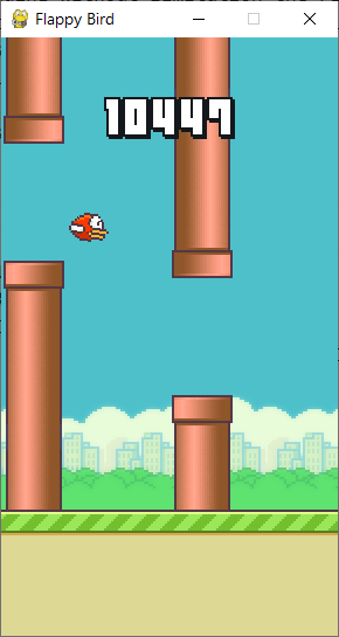
\includegraphics[width=0.8\linewidth]{figures/flappy_score.png}
\end{column}
\end{columns}
\end{frame}


\begin{frame}[fragile]{Projektvorbereitung}
\begin{columns}
\begin{column}{0.60\textwidth}
    \begin{itemize}
\item Wir starten das Spiel und spielen zunächst \textbf{manuell} ein paar Runden.

\vspace{0.5em}
\item Das Spiel benötigt das Package \textbf{pygame}. Bei Bedarf muss es nachinstalliert werden:
\vspace{0.5em}
\begin{minted}{bash}
pip install pygame
\end{minted}

\end{itemize}
\end{column}

\begin{column}{0.35\textwidth}
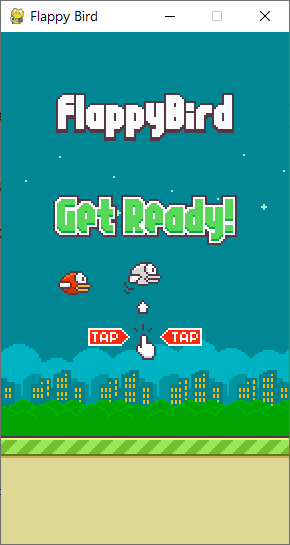
\includegraphics[width=0.8\linewidth]{figures/flappy_start.png}
\end{column}
\end{columns}
\end{frame}

\begin{frame}{Anbindung des Agenten}
\small
\begin{columns}
\begin{column}{0.47\textwidth}
Wir entfernen den \textbf{Start-} und den \textbf{Ende-Bildschirm}, damit der Agent endlos ein Spiel nach dem anderen spielen kann.

\vspace{0.5em}
Der Agent wird über zwei \textbf{Callback-Funktionen} eingebunden:
\begin{itemize}
\item \textbf{isAgentKeyPress()} übermittelt in jedem Frame den aktuellen Zustand und fragt, ob der Agent flattern will.
\item \textbf{onGameOver()} übermittelt, dass und wie der Agent gestorben ist.
\end{itemize}
\end{column}
\begin{column}{0.48\textwidth}
\includesvg[width=\linewidth]{figures/flappy_skizze.svg}
\end{column}
\end{columns}
\end{frame}

\begin{frame}{Q-Learning umsetzen}
\begin{columns}
\begin{column}{0.47\textwidth}
\begin{block}{Der aktuelle \textbf{Zustand} enthält...}
\begin{itemize}
\item die \textbf{y-Geschwindigkeit} des Vogels,
\item die \textbf{x-Position} der nächsten Röhre,
\item den \textbf{y-Abstand} zwischen Vogel und Röhre.
\end{itemize}
\end{block}
\end{column}
\begin{column}{0.48\textwidth}
\begin{blockC2}{Belohnungssystem}
\begin{itemize}
\item Überlebt der Vogel einen Frame, erhält er einen \textbf{Bonus-Punkt}.
\item Stirbt er, erhält er \textbf{-10000} Punkte Strafe.
\end{itemize}
\end{blockC2}
\end{column}
\end{columns}
\source{\cite{seemann2024mlaz}}
\end{frame}


\begin{frame}[fragile]{Lernfortschritt}
\begin{minted}[fontsize=\tiny, breaklines=true]{text}
Spiel: 200, Mittlerer Score: 0.0
[0, 0, 0, 0, 0, 0, 0, 0, 0, 0, 0, 0, 0, 0, 0, 0, 0, 0, 0, 0, 0, 0, 0, 0, 0, 0, 0, 0, 0, 0, 0, 0, 0, 0, 0, 0, 0, 0, 0, 0, 0, 0, 0, 0, 0, 0, 0, 0, 0, 0, 0, 0, 0, 0, 0, 0, 0, 0, 0, 0, 0, 0, 0, 0, 0, 0, 0, 0, 0, 0, 0, 0, 0, 0, 0, 0, 0, 0, 0, 0, 0, 0, 0, 0, 0, 0, 0, 0, 0, 0, 0, 0, 0, 0, 0, 0, 0, 0, 0, 0]

Spiel: 7500, Mittlerer Score: 0.63
[3, 0, 4, 1, 0, 0, 0, 1, 0, 1, 0, 0, 1, 4, 1, 0, 3, 0, 0, 0, 0, 0, 0, 0, 0, 1, 0, 1, 0, 1, 0, 0, 0, 0, 0, 0, 0, 5, 0, 1, 0, 0, 1, 0, 0, 1, 0, 4, 0, 0, 0, 0, 2, 0, 1, 0, 0, 0, 0, 1, 0, 2, 1, 0, 1, 0, 0, 3, 1, 0, 0, 0, 0, 3, 1, 0, 0, 0, 1, 1, 0, 1, 0, 1, 0, 0, 0, 0, 2, 0, 0, 0, 0, 1, 4, 0, 2, 0, 0, 0]

Spiel: 27300, Mittlerer Score: 49.17
[98, 86, 0, 4, 7, 146, 34, 76, 63, 171, 92, 0, 32, 46, 89, 35, 47, 36, 57, 31, 38, 13, 45, 18, 103, 62, 11, 67, 4, 76, 44, 5, 98, 63, 94, 37, 19, 32, 20, 12, 101, 41, 41, 42, 20, 51, 18, 87, 54, 77, 72, 37, 6, 82, 42, 10, 2, 168, 32, 116, 18, 119, 59, 25, 4, 0, 24, 15, 18, 80, 27, 37, 0, 198, 49, 16, 56, 30, 10, 140, 9, 72, 29, 140, 30, 10, 14, 10, 34, 34, 137, 121, 29, 13, 13, 0, 6, 57, 100, 24]

Spiel: 86000, Mittlerer Score: 73.53
[65, 28, 29, 38, 20, 11, 72, 7, 14, 66, 79, 21, 112, 53, 420, 24, 94, 118, 28, 13, 44, 132, 24, 54, 18, 175, 220, 168, 14, 173, 34, 93, 22, 37, 59, 64, 140, 25, 118, 193, 27, 42, 86, 53, 49, 58, 5, 50, 107, 8, 61, 10, 43, 13, 132, 18, 276, 9, 75, 66, 87, 222, 18, 68, 225, 227, 28, 66, 109, 2, 46, 115, 92, 120, 48, 182, 83, 0, 92, 57, 67, 45, 11, 16, 60, 7, 54, 50, 23, 24, 22, 384, 3, 1, 12, 40, 146, 58, 126, 10]

Spiel: 161000, Mittlerer Score: 3251.75
[1405, 3346, 5369, 4556, 1699, 2630, 172, 1912, 1117, 602, 3254, 9246, 1818, 1164, 558, 1902, 5425, 1502, 4625, 1311, 1930, 7352, 6016, 1132, 6630, 2394, 332, 8034, 1477, 3905, 5182, 1578, 2766, 7210, 3570, 6262, 6746, 2390, 0, 9253, 1275, 1466, 1407, 964, 4755, 1775, 2081, 3592, 320, 2304, 1609, 2628, 3983, 17331, 4030, 1076, 78, 1292, 7482, 3804, 4216, 1110, 9940, 1434, 4342, 838, 8511, 200, 4927, 1112, 100, 2006, 2125, 2573, 3912, 5528, 1193, 2857, 593, 2042, 573, 8210, 3254, 282, 6632, 2023, 487, 198, 10884, 5644, 2202, 1625, 1764, 3654, 5502, 7312, 1342, 1630, 948, 426]
\end{minted}
\end{frame}

\begin{frame}{Lernfortschritt}
\centering
\begin{tikzpicture}
\begin{axis}[
  width=0.95\textwidth,
  height=0.7\textheight,
  xlabel={Lern-Iterationen},
  ylabel={Score (Durchschnitt)},
  xmin=0, xmax=205000,
  ymin=0,
  scaled x ticks=false,
  xtick={0,50000,100000,150000,200000},
  xticklabel style={/pgf/number format/1000 sep=\,},
  yticklabel style={/pgf/number format/1000 sep=\,},
  grid=major,
  grid style={gray!25},
  tick align=outside,
  axis lines=left,
  every axis plot/.append style={very thick},
  clip=false
]
\addplot[
  draw=AccentColor,
  mark=*,
  mark size=1.6pt,
  mark options={fill=PrimaryColor, draw=PrimaryColor},
  fill=AccentColor!12,
  fill opacity=0.6
] coordinates {
  (10000,4.3) (20000,27) (30000,39) (40000,52) (50000,42)
  (60000,50) (70000,58) (80000,74) (90000,73) (100000,4)
  (110000,9) (120000,14) (130000,2) (140000,5) (150000,2331)
  (160000,3602) (170000,3488) (180000,3219) (190000,3340) (200000,2919)
} \closedcycle;
\end{axis}
\end{tikzpicture}

\vspace{0.3em}
\footnotesize
Nach einer langen Phase geringer Scores gelingt ab etwa \textbf{150.000 Iterationen} der \textbf{Durchbruch}.
\end{frame}


\makequestionspage{\FRAGENIMAGE}